\section{Introduction to Shell and Shell Script}

\begin{frame}{Shell}
\begin{multicols}{2}
\begin{itemize}
\item Kernel: the core of OS
\item Shell
\begin{itemize}
\item the interface for user or program to access to the OS's services
\item often refer to the CLI (Command-Line Interface) shells
\item a sort of different shells: sh, bash, zsh, fish...
\end{itemize}
\end{itemize}
\newpage
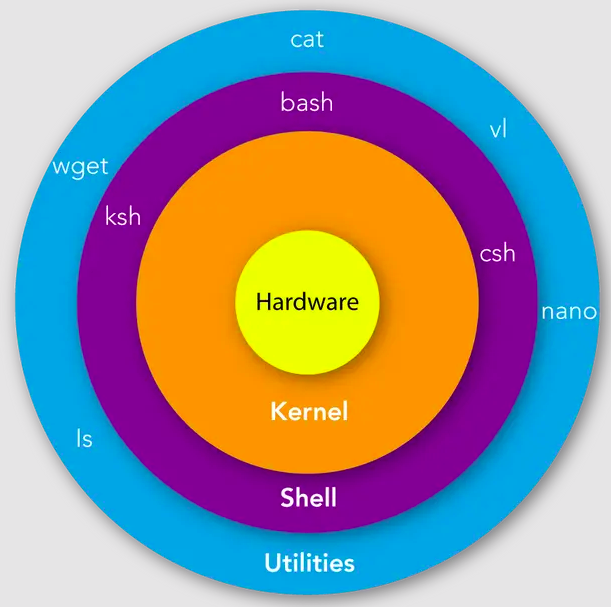
\includegraphics[width=6cm]{shell.png}\\
\tiny{(Reference: \url{https://mindmajix.com/shell-scripting-tutorial})}
\end{multicols}
\end{frame}

\begin{frame}{Bash}
\begin{itemize}
\item Bash: Bourne-Again Shell
\item Default login shell on most systems (ex: CSIE workstations)
\item Will be used in this lab, HW, and semester
\item Check your shell!\\

\includegraphics[width=5cm]{echoshell.png}
\end{itemize}
\end{frame}

\begin{frame}{Shell Script}
\begin{itemize}
\item If you want to type a lot of commands, then directly typing it in shell is inconvenience.
\item Type the commands in a file, and execute it.
\end{itemize}
\end{frame}

\section{Do Things Like A PRO}

\begin{frame}{Who to Ask}
\begin{itemize}
\item Ask the \t{man}:
\begin{itemize}
\item \t{man cmd}: show the manual page of the command \t{cmd}
\item Ex: \t{man cd}, \t{man ls}, ...
\item \t{man man} for more details
\end{itemize}
\item Ask for help:
\begin{itemize}
\item \t{cmd -h}, \t{cmd --help}
\item Ex: \t{cd --help}, \t{ls --help}
\end{itemize}
\item Ask Google or ChatGPT: will be very helpful in this class
\item \href{https://github.com/tldr-pages/tldr}{tldr} may help
\end{itemize}
\end{frame}

\begin{frame}{Editor}
\only<1>{
\begin{multicols}{2}
\begin{itemize}
\item How to edit/execute codes on workstations?
\begin{itemize}
\item VSCode (or other local editors) + scp ?
\item Learn Vim instead.
\item VIM IS THE BEST EDITOR IN THE WORLD!
\end{itemize}
\item Vim tutorial
\begin{itemize}
\item \t{vimtutor}
\item \href{https://www.openvim.com/tutorial.html}{Vim tutorial}
\end{itemize}
\item Edit \t{\sm/.vimrc} to make Vim more convenient:
\begin{itemize}
\item \t{map <F9> :w<bar>!gcc "\%"}
\item \t{map <F10> :w<bar>!./a.out}
\end{itemize}
\end{itemize}
\newpage

\includegraphics[width=5cm]{viminstead.png}\\
\end{multicols}
}\only<2>{
\begin{center}

\includegraphics[width=7cm]{exitvim.png}
\end{center}
}
\end{frame}

\begin{frame}{SSH}
\begin{itemize}
\item SSH: Secure SHell (secure for remote connection)
\item Important:
\begin{itemize}
\item Strong password
\item Give SSH key a try
\end{itemize}
\item Keywords: \t{ssh-keygen}, \t{ssh-copy-id}, \t{ssh-agent}, \t{\sm/.ssh/config}, \t{keychain}
\item Transfering file: \t{sftp}, \t{scp}
\end{itemize}
\end{frame}

